% Options for packages loaded elsewhere
\PassOptionsToPackage{unicode}{hyperref}
\PassOptionsToPackage{hyphens}{url}
\PassOptionsToPackage{dvipsnames,svgnames,x11names}{xcolor}
%
\documentclass[
]{article}
\usepackage{amsmath,amssymb}
\usepackage{lmodern}
\usepackage{iftex}
\ifPDFTeX
  \usepackage[T1]{fontenc}
  \usepackage[utf8]{inputenc}
  \usepackage{textcomp} % provide euro and other symbols
\else % if luatex or xetex
  \usepackage{unicode-math}
  \defaultfontfeatures{Scale=MatchLowercase}
  \defaultfontfeatures[\rmfamily]{Ligatures=TeX,Scale=1}
\fi
% Use upquote if available, for straight quotes in verbatim environments
\IfFileExists{upquote.sty}{\usepackage{upquote}}{}
\IfFileExists{microtype.sty}{% use microtype if available
  \usepackage[]{microtype}
  \UseMicrotypeSet[protrusion]{basicmath} % disable protrusion for tt fonts
}{}
\makeatletter
\@ifundefined{KOMAClassName}{% if non-KOMA class
  \IfFileExists{parskip.sty}{%
    \usepackage{parskip}
  }{% else
    \setlength{\parindent}{0pt}
    \setlength{\parskip}{6pt plus 2pt minus 1pt}}
}{% if KOMA class
  \KOMAoptions{parskip=half}}
\makeatother
\usepackage{xcolor}
\usepackage{graphicx}
\makeatletter
\def\maxwidth{\ifdim\Gin@nat@width>\linewidth\linewidth\else\Gin@nat@width\fi}
\def\maxheight{\ifdim\Gin@nat@height>\textheight\textheight\else\Gin@nat@height\fi}
\makeatother
% Scale images if necessary, so that they will not overflow the page
% margins by default, and it is still possible to overwrite the defaults
% using explicit options in \includegraphics[width, height, ...]{}
\setkeys{Gin}{width=\maxwidth,height=\maxheight,keepaspectratio}
% Set default figure placement to htbp
\makeatletter
\def\fps@figure{htbp}
\makeatother
\setlength{\emergencystretch}{3em} % prevent overfull lines
\providecommand{\tightlist}{%
  \setlength{\itemsep}{0pt}\setlength{\parskip}{0pt}}
\setcounter{secnumdepth}{-\maxdimen} % remove section numbering
\newlength{\cslhangindent}
\setlength{\cslhangindent}{1.5em}
\newlength{\csllabelwidth}
\setlength{\csllabelwidth}{3em}
\newlength{\cslentryspacingunit} % times entry-spacing
\setlength{\cslentryspacingunit}{\parskip}
\newenvironment{CSLReferences}[2] % #1 hanging-ident, #2 entry spacing
 {% don't indent paragraphs
  \setlength{\parindent}{0pt}
  % turn on hanging indent if param 1 is 1
  \ifodd #1
  \let\oldpar\par
  \def\par{\hangindent=\cslhangindent\oldpar}
  \fi
  % set entry spacing
  \setlength{\parskip}{#2\cslentryspacingunit}
 }%
 {}
\usepackage{calc}
\newcommand{\CSLBlock}[1]{#1\hfill\break}
\newcommand{\CSLLeftMargin}[1]{\parbox[t]{\csllabelwidth}{#1}}
\newcommand{\CSLRightInline}[1]{\parbox[t]{\linewidth - \csllabelwidth}{#1}\break}
\newcommand{\CSLIndent}[1]{\hspace{\cslhangindent}#1}
\ifLuaTeX
\usepackage[bidi=basic]{babel}
\else
\usepackage[bidi=default]{babel}
\fi
\babelprovide[main,import]{american}
% get rid of language-specific shorthands (see #6817):
\let\LanguageShortHands\languageshorthands
\def\languageshorthands#1{}
\ifLuaTeX
  \usepackage{selnolig}  % disable illegal ligatures
\fi
\IfFileExists{bookmark.sty}{\usepackage{bookmark}}{\usepackage{hyperref}}
\IfFileExists{xurl.sty}{\usepackage{xurl}}{} % add URL line breaks if available
\urlstyle{same} % disable monospaced font for URLs
\hypersetup{
  pdftitle={PyVBMC: Efficient Bayesian inference in Python},
  pdfauthor={Bobby Huggins, Chengkun Li, Marlon Tobaben, Mikko J.
Aarnos, Luigi Acerbi},
  pdflang={en-US},
  colorlinks=true,
  linkcolor={Maroon},
  filecolor={Maroon},
  citecolor={Blue},
  urlcolor={Blue},
  pdfcreator={LaTeX via pandoc}}

\title{PyVBMC: Efficient Bayesian inference in Python}

%%%%%%%%%%%%%%%%%%%%%%%%%%%%%%%%%%%%%%%%%%%%%%%%%%%%%%%%%%%%%%%%%%%%%%%%
% Authors and Affiliations

\usepackage[affil-it]{authblk}
%% \renewcommand\Authsep{, }
\setlength{\affilsep}{1em}
\author[1%
  *%
  \ensuremath\mathparagraph]{Bobby Huggins%
    \,%
    }
\author[1%
  *%
  ]{Chengkun Li%
    \,%
    }
\author[1%
  *%
  ]{Marlon Tobaben%
    \,%
    }
\author[1%
  %
  ]{Mikko J. Aarnos%
    }
\author[1%
  %
  \ensuremath\mathparagraph]{Luigi Acerbi%
    \,%
    }

\affil[1]{University of Helsinki}
\affil[$\mathparagraph$]{Corresponding author}
\affil[*]{These authors contributed equally.}
%%%%%%%%%%%%%%%%%%%%%%%%%%%%%%%%%%%%%%%%%%%%%%%%%%%%%%%%%%%%%%%%%%%%%%%%
\date{27 February 2023}

\begin{document}
\maketitle

\hypertarget{summary}{%
\section{Summary}\label{summary}}

PyVBMC is a Python implementation of the Variational Bayesian Monte
Carlo (VBMC) algorithm for posterior and model inference for
\emph{black-box} computational models
(\protect\hyperlink{ref-acerbi_variational_2018}{Acerbi, 2018},
\protect\hyperlink{ref-acerbi_variational_2020}{2020}). VBMC is an
approximate inference method designed for efficient parameter estimation
and model assessment when model evaluations are mildly-to-very expensive
(e.g., a second or more) and/or noisy. Specifically, VBMC computes:

\begin{itemize}
\tightlist
\item
  a flexible (non-Gaussian) approximate posterior distribution of the
  model parameters, from which statistics and posterior samples can be
  easily extracted;
\item
  an approximation of the model evidence or marginal likelihood, a
  metric used for Bayesian model selection.
\end{itemize}

PyVBMC can be applied to any computational or statistical model with up
to roughly 10-15 continuous parameters, with the only requirement that
the user can provide a Python function that computes the target log
likelihood of the model, or an approximation thereof (e.g., an estimate
of the likelihood obtained via simulation or Monte Carlo methods).
PyVBMC is particularly effective when the model takes more than about a
second per evaluation, with dramatic speed-ups of 1-2 orders of
magnitude when compared to traditional approximate inference methods.

Extensive benchmarks on both artificial test problems and a large number
of real models from the computational sciences, particularly
computational and cognitive neuroscience, show that VBMC generally ---
and often vastly --- outperforms alternative methods for
sample-efficient Bayesian inference, and is applicable to both exact and
simulator-based models
(\protect\hyperlink{ref-acerbi_variational_2018}{Acerbi, 2018},
\protect\hyperlink{ref-acerbi_exploration_2019}{2019},
\protect\hyperlink{ref-acerbi_variational_2020}{2020}). PyVBMC brings
this state-of-the-art inference algorithm to Python, along with an
easy-to-use Pythonic interface for running the algorithm and
manipulating and visualizing its results.

\hypertarget{statement-of-need}{%
\section{Statement of need}\label{statement-of-need}}

Standard methods for Bayesian inference over arbitrary statistical and
computational models, such as Markov Chain Monte Carlo (MCMC) methods,
traditional variational inference, and nested sampling, require a large
number of evaluations of the target density, and/or a model which is
differentiable with respect to its parameters
(\protect\hyperlink{ref-martin_computing_2020}{Martin et al., 2020};
\protect\hyperlink{ref-murphy_probabilistic_2023}{Murphy, 2023}). PyVBMC
targets problems that are not amenable to these existing approaches: It
uses no parameter gradients, so it is applicable to black-box models,
and it is \emph{sample-efficient}, requiring very few likelihood
evaluations, typically on the order of a few hundred, as opposed to the
many (tens of) thousands required by most other approximate inference
methods.

\hypertarget{method}{%
\subsection{Method}\label{method}}

PyVBMC achieves practical sample-efficiency in a unique manner by
simultaneously building two approximations of the true, expensive target
posterior distribution:

\begin{itemize}
\tightlist
\item
  A Gaussian process (GP) surrogate of the target (unnormalized) log
  posterior density.
\item
  A variational approximation --- an expressive mixture of Gaussian
  distributions with an arbitrary number of components --- fit to the GP
  surrogate.
\end{itemize}

The uncertainty-aware GP surrogate is built iteratively via active
sampling, selecting which points to evaluate next so as to explore the
posterior landscape and reduce uncertainty in the approximation
(\autoref{fig:example}). In this respect, PyVBMC works similarly to
Bayesian optimization methods
(\protect\hyperlink{ref-garnett_bayesian_2023}{Garnett, 2023}), although
with the different objective of learning the full shape of the target
posterior as opposed to only searching for the optimum of the target.

\begin{figure}
\centering
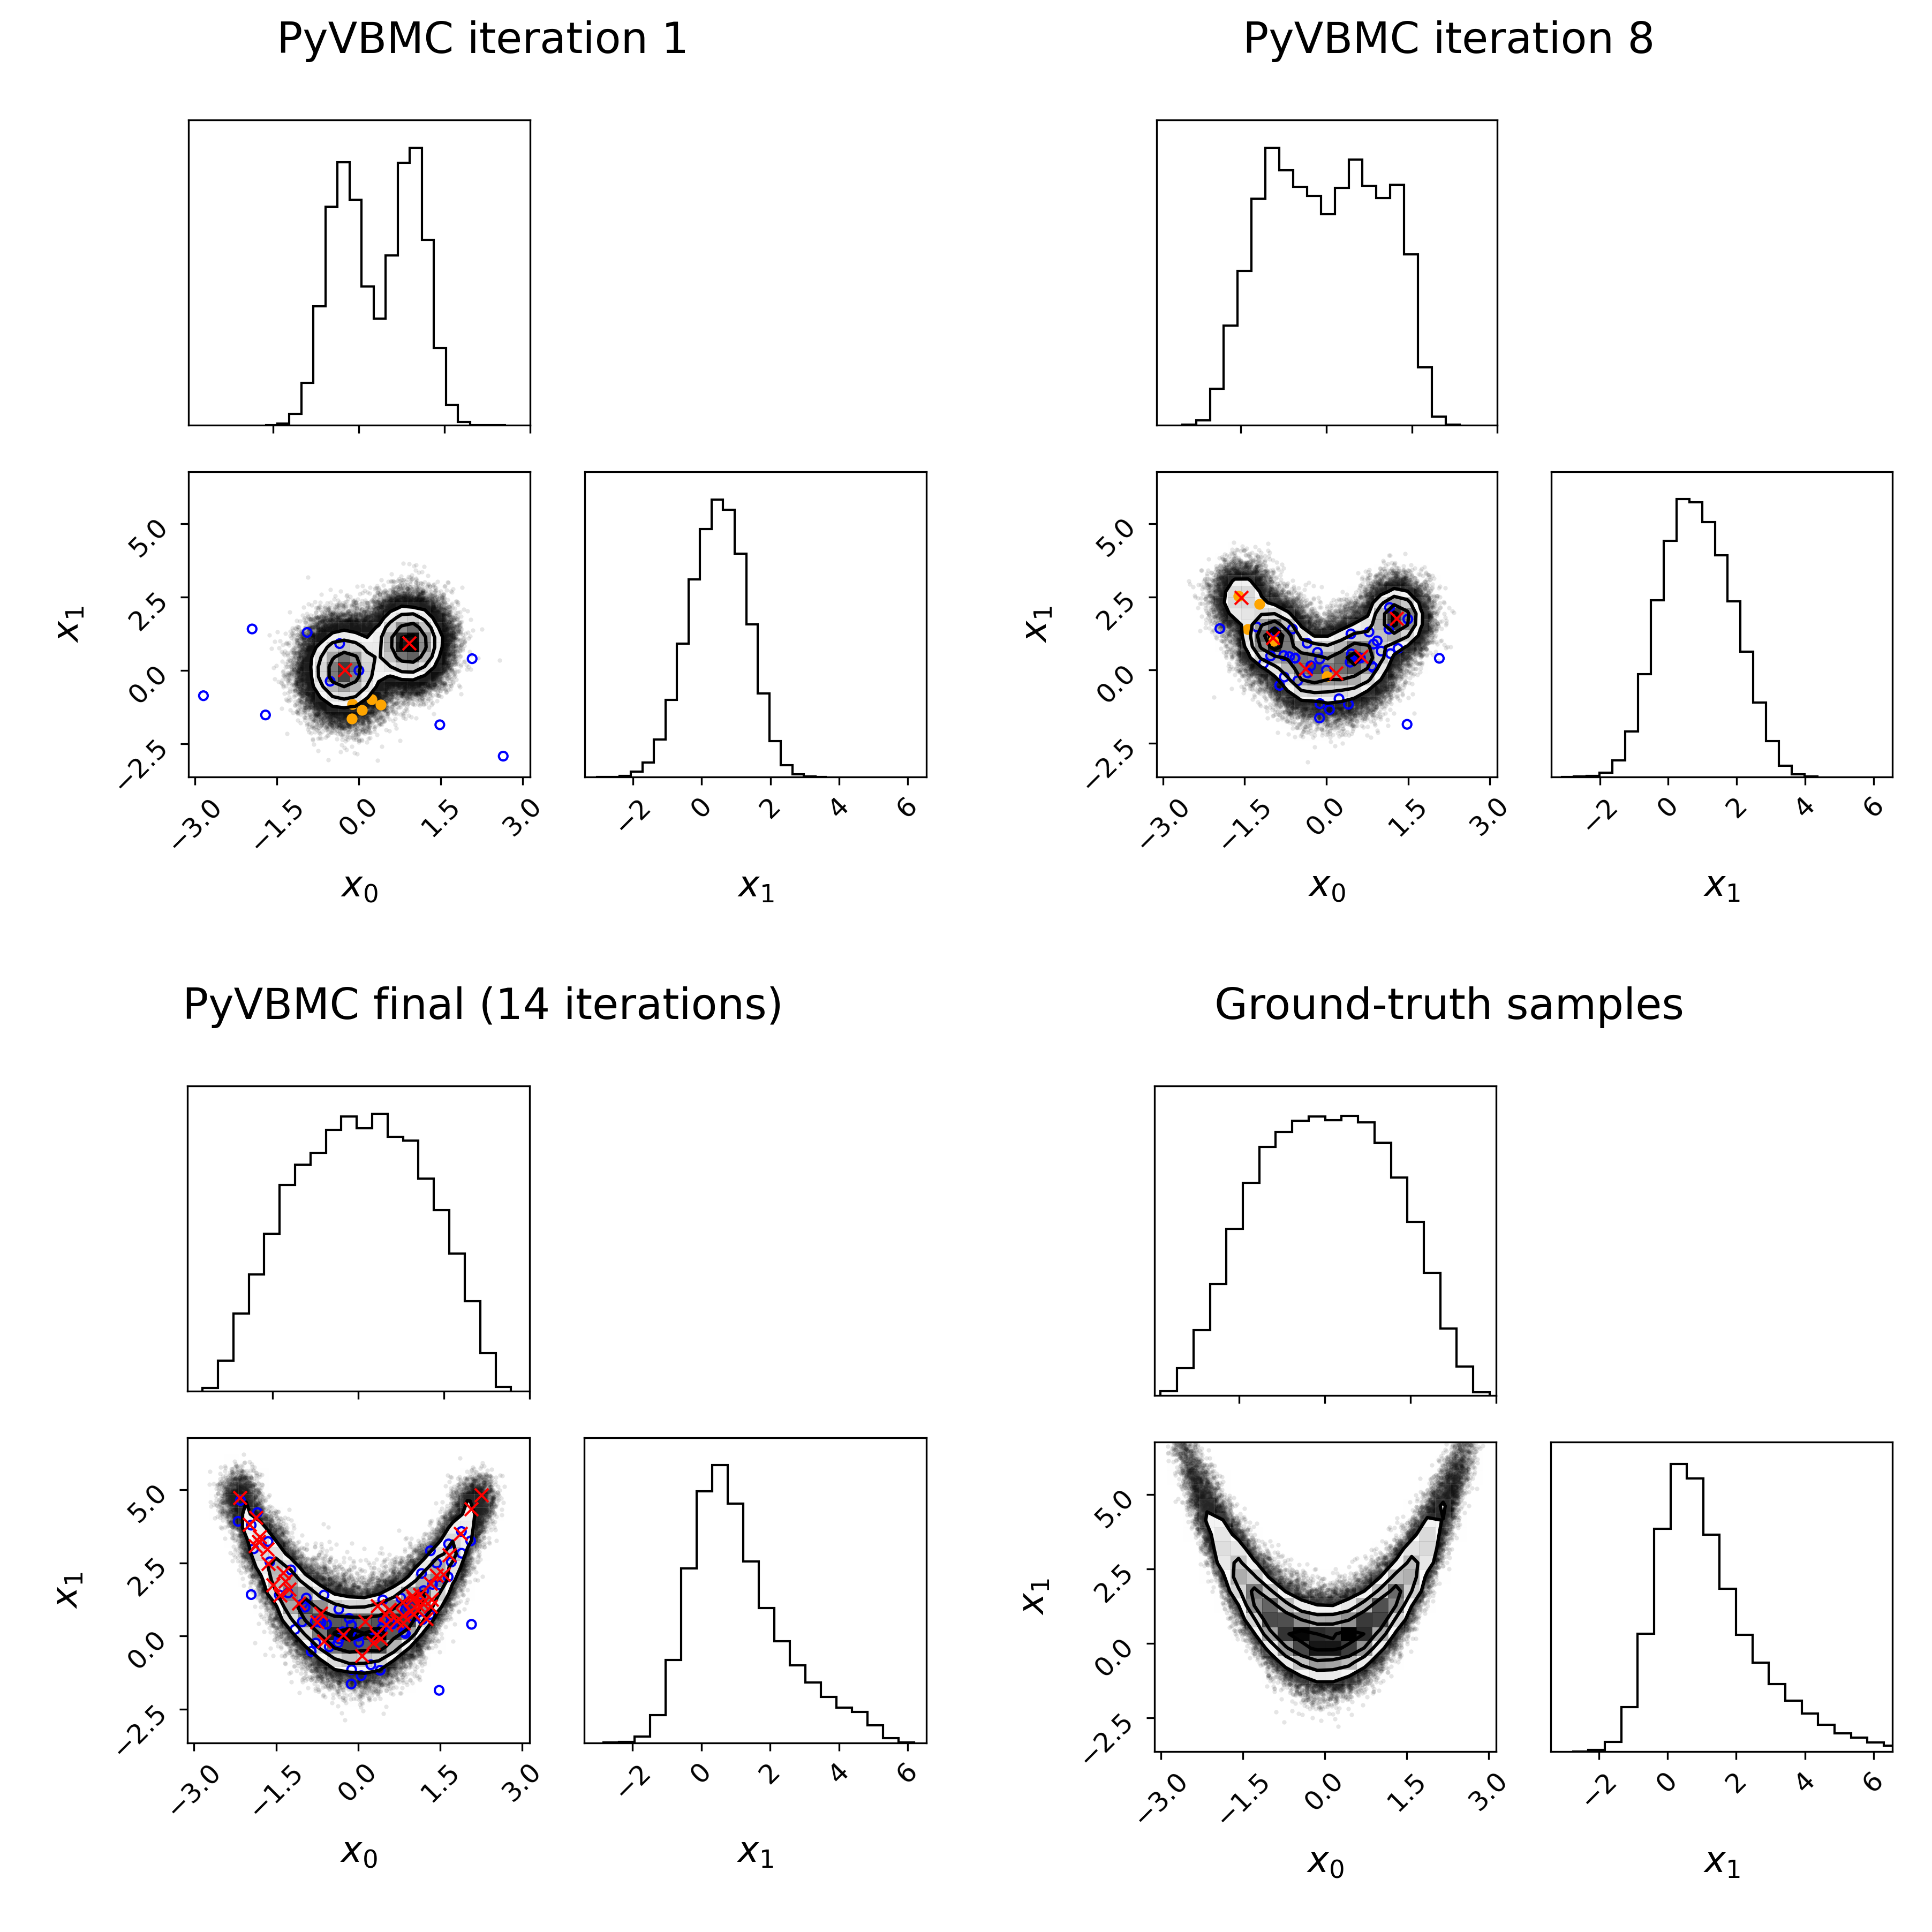
\includegraphics{combined_figures_with_gt.png}
\caption{Contour plots and marginal histograms show PyVBMC exploring a
two-dimensional posterior (a
\href{https://en.wikipedia.org/wiki/Rosenbrock_function}{Rosenbrock}
likelihood with Gaussian prior). The solid orange circles indicate new
points chosen by active sampling, the empty blue circles indicate
previously sampled points, and the red crosses indicate centers of the
variational posterior mixture components. 10 points are sampled
initially, and each iteration consists of 5 actively sampled points,
meaning that the final result is obtained with only 80 evaluations of
the target density.\label{fig:example}}
\end{figure}

At the same time, in each iteration of PyVBMC a variational
approximation is fit to the current GP surrogate by optimizing a lower
bound to the log model evidence (ELBO). This second approximation thus
provides an estimate of the normalization constant of the posterior,
useful for Bayesian model selection, and yields a tractable distribution
(a very flexible mixture of Gaussians) we can easily compute with and
draw samples from. Crucially, obtaining this variational approximation
is inexpensive because the ELBO and its gradients can be efficiently
estimated via Bayesian quadrature
(\protect\hyperlink{ref-ghahramani_bayesian_2002}{Ghahramani \&
Rasmussen, 2002}; \protect\hyperlink{ref-ohagan_bayesian_1991}{O'Hagan,
1991}), without relying on additional evaluations of the true target
posterior.

The variational approximation is a unique feature of the VBMC algorithm
that makes it particularly efficient and robust, as both the current
ELBO and the variational posterior are used throughout all steps of the
algorithm. For example: as diagnostics for convergence and stability of
the solution; to obtain a better representation of the target by
rotating the axes via \emph{variational whitening}; to estimate complex
integrated acquisition functions for active sampling with noisy targets.
All of these algorithmic steps would be cumbersome if not unfeasible
without an easy, tractable representation of the posterior at each
iteration. Notably, the GP itself is not tractable as its normalization
constant is unknown and we cannot directly draw posterior samples from
the surrogate log density: this is where the variational posterior
approximation steps in.

In practice, PyVBMC returns the final variational posterior as an object
that can be easily manipulated by the user, and an estimate of the ELBO
and of its uncertainty. Importantly, several diagnostics are
automatically applied to detect lack of convergence of the method.

\hypertarget{related-work}{%
\subsection{Related work}\label{related-work}}

Algorithms predating VBMC, such as WSABI
(\protect\hyperlink{ref-gunter_sampling_2014}{Gunter et al., 2014}), BBQ
(\protect\hyperlink{ref-osborne_active_2012}{Osborne et al., 2012}),
BAPE (\protect\hyperlink{ref-kandasamy_bayesian_2015}{Kandasamy et al.,
2015}), and AGP (\protect\hyperlink{ref-wang_adaptive_2018}{Wang \& Li,
2018}), employ similar strategies but underperform VBMC in previous
experiments, and to our knowledge are not readily available as packaged
and user-friendly software for Bayesian inference\footnote{Emukit
  (\protect\hyperlink{ref-paleyes_emulation_2019}{Paleyes et al., 2019})
  implements WSABI, but targets Bayesian optimization and
  general-purpose quadrature over inference.}. The Python package GPry
(\protect\hyperlink{ref-gammal_fast_2022}{Gammal et al., 2022}),
released after VBMC but before PyVBMC, likewise relies on surrogate
modeling and active sampling, but learns only a GP surrogate --- not a
variational posterior --- and so generating samples or estimating the
model evidence requires further post-processing.

Furthermore, neither GPry nor the aforementioned algorithms are designed
to handle noisy log density evaluations. Standard approaches to active
sampling based on a surrogate GP can be easily fooled if the model's
likelihood is not a deterministic function of the parameters, but is
instead measured only up to random error
(\protect\hyperlink{ref-jarvenpaa_parallel_2021}{Järvenpää et al.,
2021}). Noisy evaluations of the log density occur frequently in
simulator-based inference, where the likelihood is estimated from
simulated data and statistics thereof. PyVBMC includes separate defaults
and robust integrated acquisition functions for working with noisy
likelihoods and therefore is particularly well suited to noisy and
simulator-based contexts.

\hypertarget{applications-and-usage}{%
\subsection{Applications and usage}\label{applications-and-usage}}

The VBMC algorithm, in its MATLAB implementation, has already been
applied to fields as diverse as neuroscience
(\protect\hyperlink{ref-stine_differentiating_2020}{Stine et al.,
2020}), nuclear engineering
(\protect\hyperlink{ref-che_application_2021}{Che et al., 2021}),
geophysical inverse problems
(\protect\hyperlink{ref-hao_application_2022}{Hao et al., 2022}), and
cancer research
(\protect\hyperlink{ref-demetriades_interrogating_2022}{Demetriades et
al., 2022}). With PyVBMC, we bring the same sample-efficient and robust
inference to the wider open-source Python community, while improving the
interface, test coverage, and documentation.

The package is available on both PyPI (\texttt{pip\ install\ pyvbmc})
and \texttt{conda-forge}, and provides an idiomatic and accessible
interface, only depending on standard, widely available scientific
Python packages
(\protect\hyperlink{ref-foreman-mackey_corner_2016}{Foreman-Mackey,
2016}; \protect\hyperlink{ref-harris_array_2020}{Harris et al., 2020}).
The user only needs to give a few basic details about their model and
its parameter space, and PyVBMC handles the rest of the inference
process. PyVBMC runs out of the box without tunable parameters and
includes automatic handling of bounded variables, robust termination
conditions, and sensible default settings. At the same time, experienced
users can easily supply their own options. We have extensively tested
the algorithm and implementation details for correctness and
performance. We provide detailed
\href{https://github.com/acerbilab/pyvbmc/tree/main/examples}{tutorials},
so that PyVBMC may be accessible to those not already familiar with
approximate Bayesian inference, and our comprehensive
\href{https://acerbilab.github.io/pyvbmc}{documentation} will aid not
only new users but future contributors as well.

\hypertarget{acknowledgments}{%
\section{Acknowledgments}\label{acknowledgments}}

Work on the PyVBMC package is supported by the Academy of Finland
Flagship programme: Finnish Center for Artificial Intelligence FCAI.

\hypertarget{references}{%
\section*{References}\label{references}}
\addcontentsline{toc}{section}{References}

\hypertarget{refs}{}
\begin{CSLReferences}{1}{0}
\leavevmode\vadjust pre{\hypertarget{ref-acerbi_variational_2018}{}}%
Acerbi, L. (2018). {V}ariational {B}ayesian {M}onte {C}arlo.
\emph{Advances in Neural Information Processing Systems}, \emph{31},
8222--8232.

\leavevmode\vadjust pre{\hypertarget{ref-acerbi_exploration_2019}{}}%
Acerbi, L. (2019). An exploration of acquisition and mean functions in
{V}ariational {B}ayesian {M}onte {C}arlo. \emph{PMLR}, \emph{96}, 1--10.

\leavevmode\vadjust pre{\hypertarget{ref-acerbi_variational_2020}{}}%
Acerbi, L. (2020). {V}ariational {B}ayesian {M}onte {C}arlo with noisy
likelihoods. \emph{Advances in Neural Information Processing Systems},
\emph{33}, 8211--8222.

\leavevmode\vadjust pre{\hypertarget{ref-che_application_2021}{}}%
Che, Y., Wu, X., Pastore, G., Li, W., \& Shirvan, K. (2021). Application
of kriging and {Variational Bayesian Monte Carlo} method for improved
prediction of doped UO2 fission gas release. \emph{Annals of Nuclear
Energy}, \emph{153}, 108046.
https://doi.org/\url{https://doi.org/10.1016/j.anucene.2020.108046}

\leavevmode\vadjust pre{\hypertarget{ref-demetriades_interrogating_2022}{}}%
Demetriades, M., Zivanovic, M., Hadjicharalambous, M., Ioannou, E.,
Ljujic, B., Vucicevic, K., Ivosevic, Z., Dagovic, A., Milivojevic, N.,
Kokkinos, O., Bauer, R., \& Vavourakis, V. (2022). Interrogating and
quantifying in vitro cancer drug pharmacodynamics via agent-based and
{Bayesian} {Monte Carlo} modelling. \emph{Pharmaceutics}, \emph{14}(4).
\url{https://doi.org/10.3390/pharmaceutics14040749}

\leavevmode\vadjust pre{\hypertarget{ref-foreman-mackey_corner_2016}{}}%
Foreman-Mackey, D. (2016). Corner.py: Scatterplot matrices in {Python}.
\emph{Journal of Open Source Software}, \emph{1}(2), 24.
\url{https://doi.org/10.21105/joss.00024}

\leavevmode\vadjust pre{\hypertarget{ref-gammal_fast_2022}{}}%
Gammal, J. E., Schöneberg, N., Torrado, J., \& Fidler, C. (2022).
\emph{Fast and robust {Bayesian} inference using {Gaussian} processes
with {GPry}}. arXiv. \url{http://arxiv.org/abs/2211.02045}

\leavevmode\vadjust pre{\hypertarget{ref-garnett_bayesian_2023}{}}%
Garnett, R. (2023). \emph{{Bayesian Optimization}}. Cambridge University
Press.

\leavevmode\vadjust pre{\hypertarget{ref-ghahramani_bayesian_2002}{}}%
Ghahramani, Z., \& Rasmussen, C. (2002). {Bayesian Monte Carlo}. In S.
Becker, S. Thrun, \& K. Obermayer (Eds.), \emph{Advances in neural
information processing systems} (Vol. 15). MIT Press.
\url{https://proceedings.neurips.cc/paper/2002/file/24917db15c4e37e421866448c9ab23d8-Paper.pdf}

\leavevmode\vadjust pre{\hypertarget{ref-gunter_sampling_2014}{}}%
Gunter, T., Osborne, M. A., Garnett, R., Hennig, P., \& Roberts, S. J.
(2014). Sampling for inference in probabilistic models with fast
{Bayesian} quadrature. In Z. Ghahramani, M. Welling, C. Cortes, N.
Lawrence, \& K. Q. Weinberger (Eds.), \emph{Advances in neural
information processing systems} (Vol. 27). Curran Associates, Inc.
\url{https://proceedings.neurips.cc/paper/2014/file/e94f63f579e05cb49c05c2d050ead9c0-Paper.pdf}

\leavevmode\vadjust pre{\hypertarget{ref-hao_application_2022}{}}%
Hao, W., Duan, R., \& Yang, K. (2022). Application of dual-source modal
dispersion and {Variational Bayesian Monte Carlo} method for local
geoacoustic inversion in weakly range-dependent shallow water.
\emph{Acoustics Australia}.
\url{https://doi.org/10.1007/s40857-022-00277-2}

\leavevmode\vadjust pre{\hypertarget{ref-harris_array_2020}{}}%
Harris, C. R., Millman, K. J., Walt, S. J. van der, Gommers, R.,
Virtanen, P., Cournapeau, D., Wieser, E., Taylor, J., Berg, S., Smith,
N. J., Kern, R., Picus, M., Hoyer, S., Kerkwijk, M. H. van, Brett, M.,
Haldane, A., Río, J. F. del, Wiebe, M., Peterson, P., \ldots{} Oliphant,
T. E. (2020). Array programming with NumPy. \emph{Nature},
\emph{585}(7825), 357--362.
\url{https://doi.org/10.1038/s41586-020-2649-2}

\leavevmode\vadjust pre{\hypertarget{ref-jarvenpaa_parallel_2021}{}}%
Järvenpää, M., Gutmann, M. U., Vehtari, A., \& Marttinen, P. (2021).
Parallel {Gaussian} process surrogate {Bayesian} inference with noisy
likelihood evaluations. \emph{Bayesian Analysis}, \emph{16}(1),
147--178. \url{https://doi.org/10.1214/20-BA1200}

\leavevmode\vadjust pre{\hypertarget{ref-kandasamy_bayesian_2015}{}}%
Kandasamy, K., Schneider, J., \& Póczos, B. (2015). {Bayesian} active
learning for posterior estimation. \emph{Proceedings of the 24th
International Conference on Artificial Intelligence}, 3605--3611.
ISBN:~9781577357384

\leavevmode\vadjust pre{\hypertarget{ref-martin_computing_2020}{}}%
Martin, G. M., Frazier, D. T., \& Robert, C. P. (2020). Computing
{Bayes}: {Bayesian} computation from 1763 to the 21st century.
\emph{arXiv: Computation}.

\leavevmode\vadjust pre{\hypertarget{ref-murphy_probabilistic_2023}{}}%
Murphy, K. P. (2023). \emph{Probabilistic {Machine} {Learning}:
{Advanced} {Topics}}. MIT Press. \url{http://probml.github.io/book2}

\leavevmode\vadjust pre{\hypertarget{ref-ohagan_bayesian_1991}{}}%
O'Hagan, A. (1991). Bayes--hermite quadrature. \emph{Journal of
Statistical Planning and Inference}, \emph{29}(3), 245--260.
https://doi.org/\url{https://doi.org/10.1016/0378-3758(91)90002-V}

\leavevmode\vadjust pre{\hypertarget{ref-osborne_active_2012}{}}%
Osborne, M., Garnett, R., Ghahramani, Z., Duvenaud, D. K., Roberts, S.
J., \& Rasmussen, C. (2012). Active learning of model evidence using
{Bayesian} quadrature. In F. Pereira, C. J. Burges, L. Bottou, \& K. Q.
Weinberger (Eds.), \emph{Advances in neural information processing
systems} (Vol. 25). Curran Associates, Inc.
\url{https://proceedings.neurips.cc/paper/2012/file/6364d3f0f495b6ab9dcf8d3b5c6e0b01-Paper.pdf}

\leavevmode\vadjust pre{\hypertarget{ref-paleyes_emulation_2019}{}}%
Paleyes, A., Pullin, M., Mahsereci, M., Lawrence, N., \& González, J.
(2019). Emulation of physical processes with {Emukit}. \emph{Second
Workshop on Machine Learning and the Physical Sciences, NeurIPS}.

\leavevmode\vadjust pre{\hypertarget{ref-stine_differentiating_2020}{}}%
Stine, G. M., Zylberberg, A., Ditterich, J., \& Shadlen, M. N. (2020).
Differentiating between integration and non-integration strategies in
perceptual decision making. \emph{eLife}, \emph{9}, e55365.
\url{https://doi.org/10.7554/eLife.55365}

\leavevmode\vadjust pre{\hypertarget{ref-wang_adaptive_2018}{}}%
Wang, H., \& Li, J. (2018). Adaptive {Gaussian} process approximation
for {Bayesian} inference with expensive likelihood functions.
\emph{Neural Computation}, \emph{30}(11), 3072--3094.
\url{https://doi.org/10.1162/neco_a_01127}

\end{CSLReferences}

\end{document}
